% This file is isea.tex.  It contains the formatting instructions for and acts as a template for submissions to ISEA 2015.  It is based on the ICCC  formats and instructions.  It uses the files isea.sty, isea.bst and isea.bib, the first two of which also borrow from AAAI IJCAI formats and instructions.
% Modified from ICCC.tex by B. Bogart

\documentclass[letterpaper]{article}
\usepackage{isea}
\usepackage[pdftex]{graphicx}
\usepackage{times}
\usepackage{helvet}
\usepackage{courier}
\usepackage[numbers]{natbib}
\usepackage[normalem]{ulem}
\useunder{\uline}{\ul}{}
\pdfinfo{
/Title (The Anatomy of Networking in High-Frequency Trading)
/Author (Peter P. Waskiewicz Jr)}
% The file isea.sty is the style file for ISEA 2015 proceedings.
%
\title{The Anatomy of Networking in High-Frequency Trading}
\author{Peter P. Waskiewicz Jr. (PJ) \\ Jump Trading \\ Chicago, IL, USA \\ pwaskiewicz@jumptrading.com
\newline
\newline
}
\setcounter{secnumdepth}{0}

\begin{document} 
\maketitle
\begin{abstract}
Networking has always served a number of very diverse environments. From Enterprise to the Cloud, Telco and edge, networking technologies have been able to use a “some sizes fit most” approach. This is good when it comes to supporting these technologies in the Linux kernel.

More specialized environments, such as High-Frequency Trading (HFT), have radically different networking requirements. Depending on the use case, one requirement might be that latency is paramount when interfacing with the market exchanges. Another use case might be in the HPC environment, where latency is still paramount, but sustained and reliable throughput is a must across grid networks.

This talk is intended to highlight where the Linux kernel networking stack intersects these requirements for HFT, and where it does not. It will also expand on how latency and jitter within HFT systems compare to “traditional” networking environments. Ultimately this talk is intended to generate discussion where HFT networking needs can help improve the existing intersection points in the kernel, and discuss where further native integration could be achieved.
\end{abstract}

\section{Keywords}

networking, kernel, xdp, offloads, trading, finance, performance

\section{Introduction}
Networking technologies have always been the most complex pieces of a modern computing system. Some technologies focus on general network connectivity, such as supporting a mobile device or personal computer, and some technologies focus on Software-Defined Networks, stitching together countless virtual machines and containers within data centers.
\newline
\newline
Modern operating systems, such as Linux, have evolved over many years to include very robust network stacks to serve these very diverse needs. Linux has found great success in adoption and datacenter footprint mainly due to the diversity and robustness of its network stack. It powers the majority of the largest Cloud Service Providers in the world, many Enterprise-level deployments, and is behind the largest install-base of handheld OS's in use today, Android.
\newline
\newline
Even with all of this diversity and flexibility, there are still environments where the Linux network stack sacrifices targeted performance for this flexibility. High-Frequency Trading environments, within the Finanical Tech world, have some fairly unique requirements for network behavior and performance.
\newline
\newline
This paper will focus on how HFT networking requirements match up against the diverse network stack capabilities of Linux. It will dive into:
\begin{itemize}
\item How synthentic benchmarking of traditional networks stack up to real-world benchmarks of traditional networks
\item How the synthetic benchmarking resembles the beginning of HFT networking requirements in practice
\item Analyzing what limitations the Linux network stack has compared to current HFT requirements for predictable latencies, and what might be done about it
\item Exploring additional aspects of HFT networking requirements that encompass High-Performance Computing (HPC) grid environments, and how the Linux network stack compares to those requirements
\end{itemize}
\let\thefootnote\relax\footnotetext{The views expressed in this paper are the author's only, and should not be attributed to Jump Trading.}
\section{"Traditional Networking", and the Synthetic Benchmarking Problem}
Networking technology is one that fits into every modern workload in some fashion. In more "traditional" settings, such as datacenter-based networks (Enterprise), or disaggregated networks (Cloud), trying to nail down performance can be a difficult task. Very diverse environments create unpredictable workloads and interrupts that can introduce large amounts of jitter. When trying to benchmark these workloads, the benchmarking tests must be fairly synthetic to reduce or eliminate much of this jitter. But herein lies the issue; the benchmarks don't capture what happens in a production setting.
\subsection{Benchmarking Setup}
All benchmarks were captured via \texttt{netperf} using the \texttt{TCP\_RR} test. The system-under-test (SUT) is an Intel\textsuperscript{\textregistered} Xeon\textsuperscript{\textregistered} ES-2640 with a Broadcom bnx2x 10GbE adapter running stock Fedora 36.  The peer system is an Intel\textsuperscript{\textregistered} Xeon\textsuperscript{\textregistered} Platinum 8180 with an Intel\textsuperscript{\textregistered} 82599ES 10GbE adapter, running Gentoo Linux.  The two systems are connected to a Mellanox SN2100 switch via Direct-Attach Twinax cables.
\subsection{Benchmark 1: Real-World Configuration}
The simplest benchmark to run is one without any tuning.  As one might expect, the results don't look terribly great.
\newline

\begin{figure}[h]
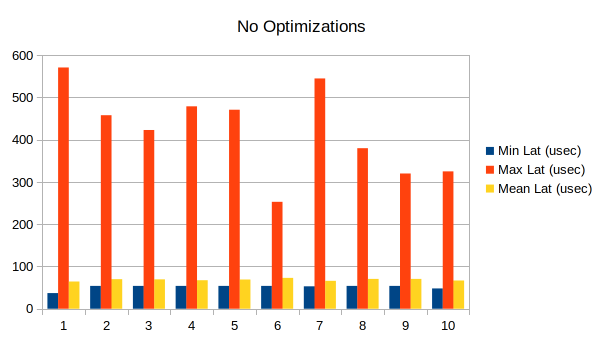
\includegraphics[width=3.31in]{netperf-no-opt.png}
\caption{Netperf with no optimizations}
\label{netperf-no-opt}
\end{figure}

As seen in Figure \ref{netperf-no-opt}, it can be observed that every run produced drastically different latency figures.

\section{Conclusion}
Coming

\section{Acknowledgments}
I would like to acknowledge the NetDev 0x16 program committee for the opportunity to submit and invitation to present this paper.

\bibliographystyle{pj-netdev-0x16}
\bibliography{pj-netdev-0x16}

\section{Author Biography}
Peter Waskiewicz Jr (PJ) is a Senior Software Engineer in Jump Trading's core engineering division, focusing on Linux kernel and device driver development, along with other system-level engineering.  Prior to Jump Trading, PJ spent the majority of his career at Intel, where he was responsible for writing and maintaining several of the Intel Ethernet Linux device drivers, and developing Linux kernel changes for scaling to 10GbE and beyond.  PJ was also a Senior Principal Engineer at NetApp in the SolidFire division, where he was the chief Linux kernel and networking architect for the SolidFire scale-out cloud storage platform. He is also an adjunct faculty at Portland State University, teaching OS and Device Drivers in the Electrical and Computer Engineering Department.

\end{document}
